%% LyX 2.1.1 created this file.  For more info, see http://www.lyx.org/.
%% Do not edit unless you really know what you are doing.
\documentclass[12pt,english]{article}
\usepackage[T1]{fontenc}
\usepackage[latin9]{inputenc}
\usepackage[a4paper]{geometry}
\geometry{verbose,tmargin=1.25cm,bmargin=1.25cm,lmargin=1.25cm,rmargin=1.25cm,headheight=1.25cm,headsep=1.25cm,footskip=1.25cm}
\usepackage{graphicx}
\usepackage{babel}
\begin{document}

\title{Week 2:FDM Applied to Solve Laplace Equation\\
for Systems with Finite Boundary Conditions}


\author{Sankeerth.D\\
EE13B102\\
Electrical Engineering}
\maketitle
\begin{abstract}
Finite Difference Method (FDM) has been used to solve the capacitor
problem in various configurations. These can be used to further model
the parasitic capacitances that occur in integrated circuits between
the interconnects and the substrate.
\end{abstract}

\section{Introduction}

FDM approximates the second derivative at a point as the average of
the four surrounding points. At the boundary, the V can be updated
using either the Dirichlet or the Neumann boundary condition. For
conductors, one can use the dirichlet conditions, and for boundaries
far away from the capacitor system, Neumann boundary condition, (gradient
being zero) can be applied.


\section{Simple capacitor cross section segment}

In this case, a close up of the cross section of the capacitor has
been considered and Neumann conditions (set to 0) have been applied
at the edges. As a result, no fringing in the field can be observed.
Dirichlet conditions of +10V and 0V have been applied on the top and
bottom plate of the capacitor, and laplace equation has been solved.

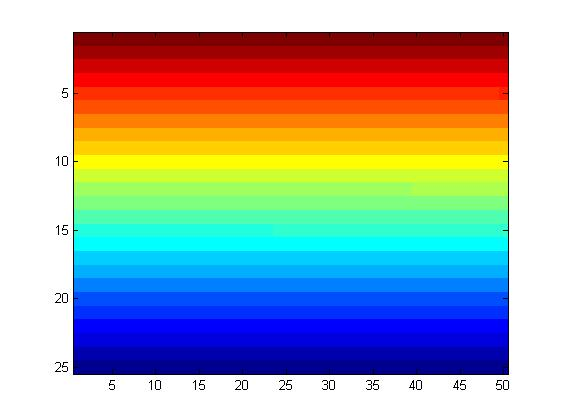
\includegraphics{prob1} 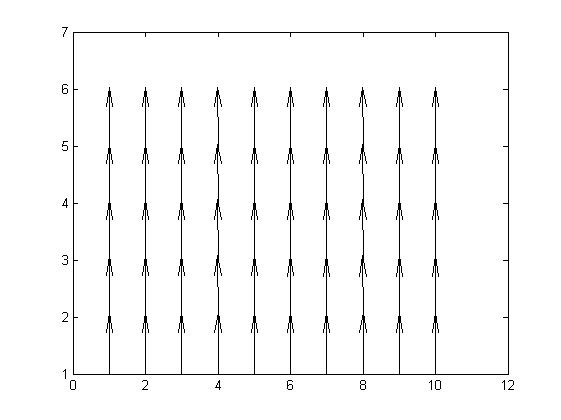
\includegraphics{prob1_field}


\section{Parallel Plate Capacitor}

Fringing can be observed in this configuration as we have considered
several times the capacitor plates' length to be the boundary. The
results (Equipotential lines) can be observed as follows:

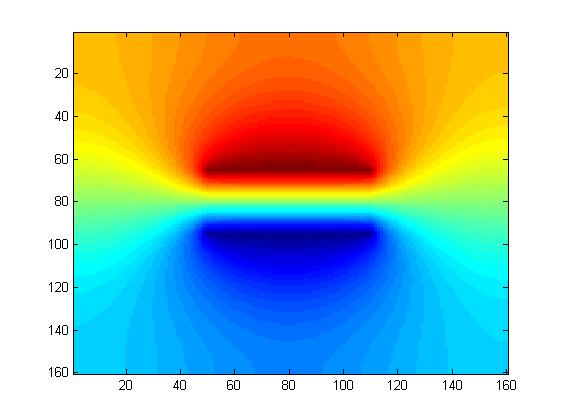
\includegraphics{prob2} 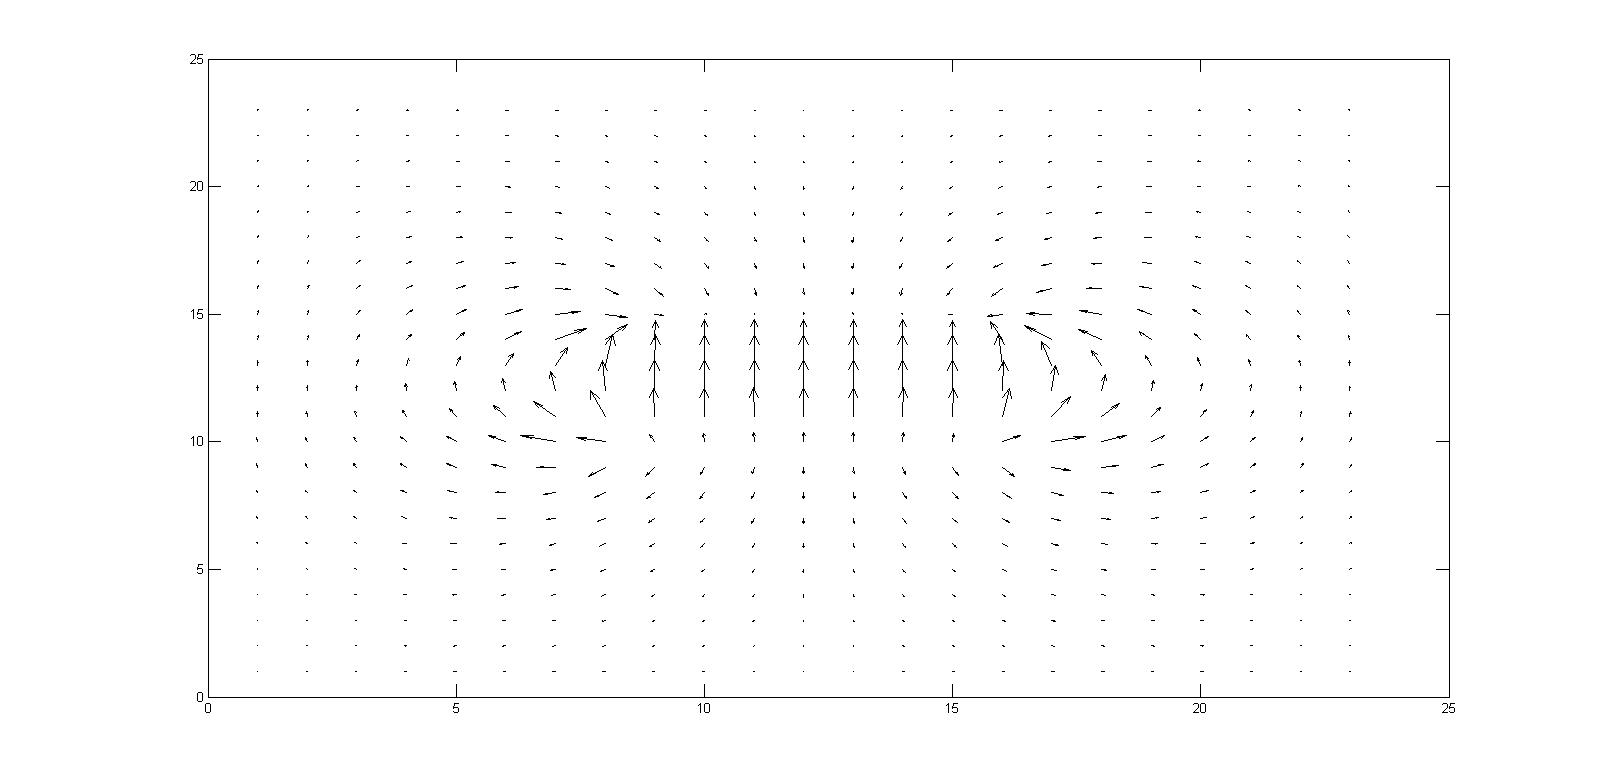
\includegraphics{prob2_field}


\section{Capacitor with one plate larger}

The upper plate is 0.1 times as large as the lower plate. as a result,
most of the higher voltage is only very near to the upper plate. One
can observe the field lines pointing along the dielectric's width.
The field has been normallized as the actual values are too small
to be visualize. Hence the field inthe middle can't be seen very clearly. 

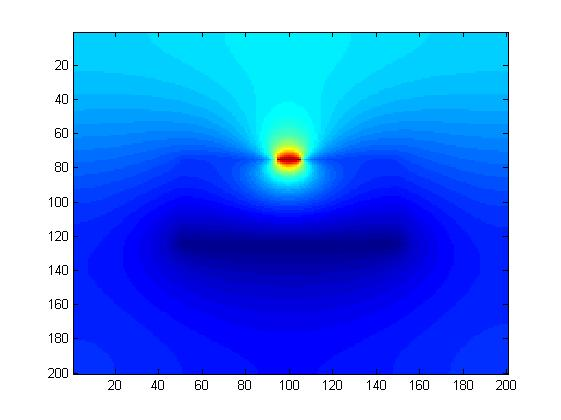
\includegraphics{prob3} 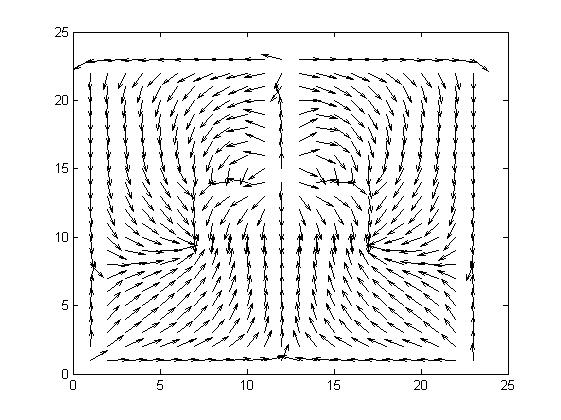
\includegraphics{prob3_field}


\section{Two separate plates with ground at the bottom}

One 10V plate is kept on the top left of the dielectric and a ground
plate to the right. Some field lines can be seen to go between the
interconnects.

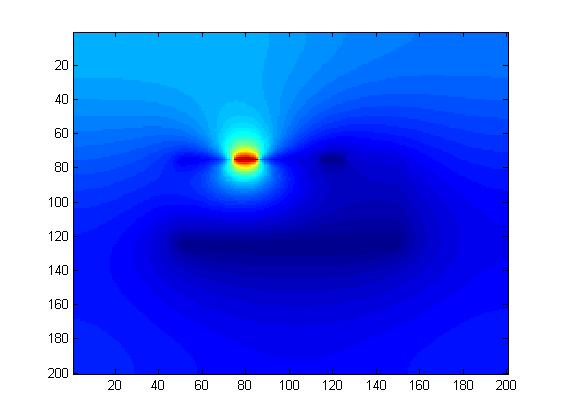
\includegraphics{prob4} 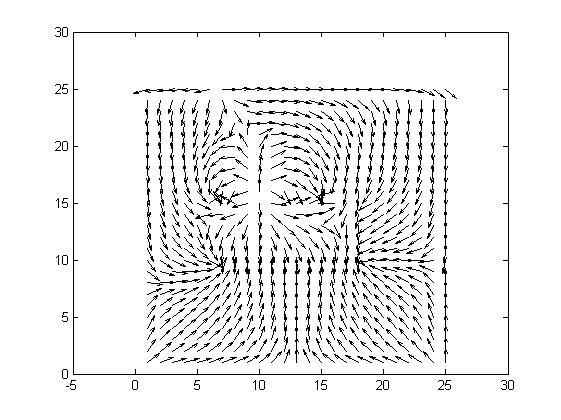
\includegraphics{prob5_field}


\section{Microstrip Capacitance}

The field structure is given as follows:

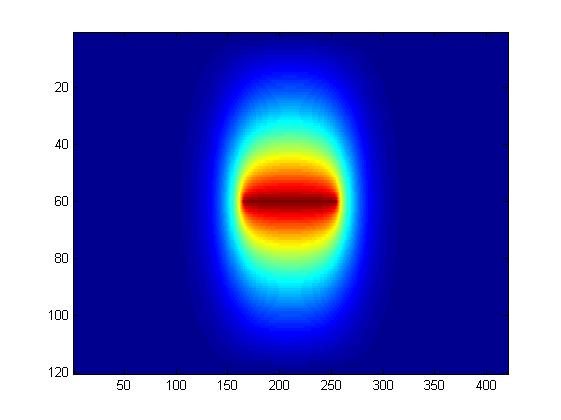
\includegraphics{microstrip} 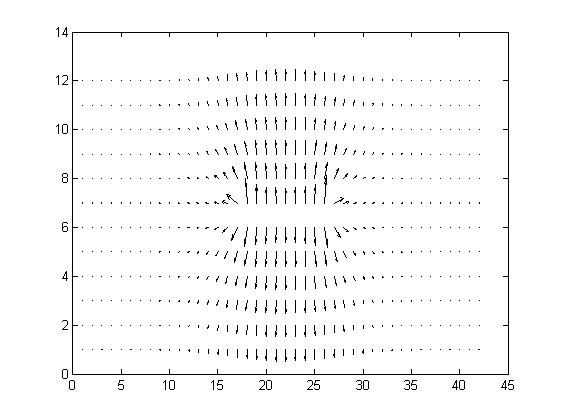
\includegraphics{mictrostrip_field}


\section{Observation}

The microstrip has a epsilon\_real = C/Cair ratio of 5.300 for w =
1.5. For 2000 as maximum number of iterations, the grid unit length
N vs Z0 (normallized) plot is as shown(almost linear):

\includegraphics{\string"plot N vs Z\string".jpg}

Also, As we increase the oteration count, we get closer and converge
towards a value for Z0. The I vs Z0 plot is as follows:

\includegraphics{\string"I vs Z\string".jpg}


\section{Result and Discussion}

The electrostatic field configuration for various capacitor configuration
has been obtained, and the general trend in field lines can be verified.
\end{document}
